\documentclass{article}
\usepackage[utf8]{inputenc}
\usepackage[T1]{fontenc}
\usepackage{amsmath}
\usepackage{tikz}

\begin{document}

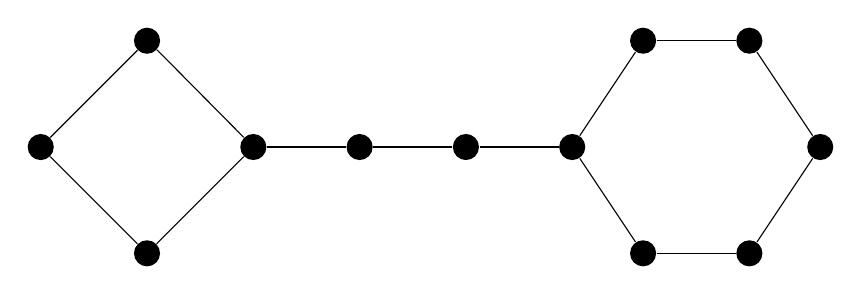
\begin{tikzpicture}  
  [scale=0.9,auto=center]
   \tikzset{dark/.style={circle,fill=black}}% here, node/.style is the style pre-defined, that will be the default layout of all the nodes. You can also create different forms for different nodes.  

 \node[dark] (d1) at (0,1.5){} ;  
  \node[dark] (d2) at (1.5,0)  {}; 
  \node[dark] (d3) at (3,1.5)  {};  
  \node[dark] (d4) at (1.5,3) {};  
   \node[dark] (d5) at (4.5,1.5)  {}; 
   \node[dark] (d6) at (6,1.5)  {}; 
   \node[dark] (d7) at (7.5,1.5)  {}; 

   \node[dark] (d8) at (8.5,3){} ;  
  \node[dark] (d9) at (8.5,0)  {}; 
  
  \node[dark] (d10) at (10,3)  {};  
  \node[dark] (d11) at (10,0) {};  
  
   \node[dark] (d12) at (11,1.5)  {}; 
  
  
 
   \draw (d1) -- (d2);
  \draw (d2) -- (d3);  
  \draw (d3) -- (d4);  
  \draw (d4) -- (d1);  
  \draw (d3) -- (d5);
  \draw (d5) -- (d6);
  \draw (d6) -- (d7);
   \draw (d7) -- (d8);
  \draw (d8) -- (d10);  
  \draw (d10) -- (d12);  
  \draw (d12) -- (d11);  
  \draw (d11) -- (d9);
  \draw (d9) -- (d7);
 

  

\end{tikzpicture}

\end{document}